Some brief notes before the problems:
\begin{itemize}
    \item \color{brickred}{Koralov and Sinai use $\times$ instead of $\otimes$ for the product $\sigma$-algebra. Moving forward, the reader needs to be cautious about what the operands are. For if they are $\sigma$-algebras, we understand the result of the expression to be the aforementioned product.} 
\end{itemize}
\begin{problem}{1}
    Find the probability that there are exactly three heads after five tosses of a symmetric coin.
\end{problem}
\begin{solution}
    Directly apply the definition of the binomial distribution. Let $X = \{0,1\}$. Define the random variable $\chi_i(\omega)$ for $1\leq i\leq 5$ to be 1 if $\omega = 1$ and zero otherwise. Then, let $\nu_5 = \sum_{i=1}^5 \chi_i$. $\nu_5$ is a binomial random variable. Thus,
    \begin{align*}
        \Pr[\nu_5 = 3] &= \binom{5}{3} \frac{1}{2^5} = \frac{5}{16}.
    \end{align*}
\end{solution}
\begin{problem}{2}
    Andrew and Bob are playing a game of table tennis. The game ends when the first player reaches 11 points if the other player has 9 points or less. However, if at any time the score is 10:10, then the game continues until one of the players is 2 points ahead. The probability that Andrew wins any given points is 60 percent. What is the probability that Andrew will go on to win the game if he is currently ahead 9:8.
\end{problem}
\begin{solution}
    We present two alternative ways to solve this problem one involving chains and the other geometric series. We first present the solution involving chains. We draw the state space below, where each node denotes a distinct score and the edges between states represent the transition probabilities
    \begin{center}
        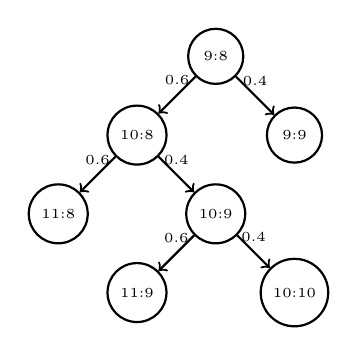
\begin{tikzpicture}[
            n/.style={draw, circle, minimum size=0.7cm, thick},
            p/.style={->, thick}
        ]
            \node[n] (a) at (0,0) {\tiny 9:8};
            \node[n] (b) at (-1,-1) {\tiny 10:8};
            \node[n] (c) at (-2,-2) {\tiny 11:8};
            \node[n] (d) at (0,-2) {\tiny 10:9};
            \node[n] (e) at (-1,-3) {\tiny 11:9};
            \node[n] (f) at (1,-3) {\tiny 10:10};
            \node[n] (g) at (1,-1) {\tiny 9:9};
            \draw[p] (a) -- node[above] {\tiny 0.6} (b);
            \draw[p] (b) -- node[above] {\tiny 0.6} (c);
            \draw[p] (b) -- node[above] {\tiny 0.4} (d);
            \draw[p] (d) -- node[above] {\tiny 0.6} (e);
            \draw[p] (d) -- node[above] {\tiny 0.4} (f);
            \draw[p] (a) -- node[above] {\tiny 0.4} (g);
        \end{tikzpicture}
        \qquad\qquad
        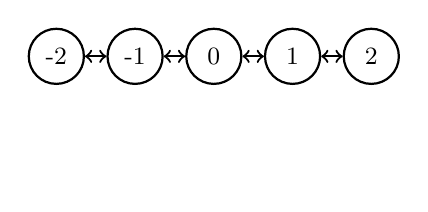
\begin{tikzpicture}[
            n/.style={draw, circle, minimum size=0.7cm, thick},
            p/.style={<->, thick}
        ]
            \node[n] (0) at (0,1.5) {\small 0};
            \node[n] (1) at (1,1.5) {\small 1};
            \node[n] (2) at (2,1.5) {\small 2};
            \node[n] (-1) at (-1,1.5) {\small -1}; 
            \node[n] (-2) at (-2,1.5) {\small -2};
            \draw[p] (0) -- (1);
            \draw[p] (1) -- (2);
            \draw[p] (0) -- (-1);
            \draw[p] (-1) -- (-2);
            \node at (0,0) {};
        \end{tikzpicture}
    \end{center}
    It remains to find the probability that Andrew wins from either 9:9 or 10:10 which is the same since both states require Andrew to win two consecutive points. This, then induces a new chain (see above). Denote by $a,b,c$ the probability that Andrew wins from being one point down, drawn, and one point up. Then, 
    \begin{align*}
        a &= 0.6b, \\
        b &= 0.4a + 0.6c, \\
        c &= 0.4b + 0.6b.
    \end{align*}
    So, $c = 0.36/0.52$. Thus, the probability that Andrew wins is then the aggregate of all states in the chain multiplied by their transition probabilities:
    \[
        \Pr[\text{Andrew wins}] = 0.4\left(\frac{0.36}{0.52}\right) + 0.6\left(0.6 + 0.4\left(0.4\left(\frac{0.36}{0.52}\right) + 0.6\right)\right) = 0.847.  
    \]
\end{solution}
\begin{problem}{3}
    Will you consider a coin asymmetric if after 1000 coin tosses the number of heads is equal to 600?
\end{problem}
\begin{solution}
    We directly apply the de Moivre-Laplace Theorem. Let $X_i(\omega_i)$ be a random variable that is 1 if $\omega_i =\text{heads}$ and 0 otherwise. Then, let $\nu_n = \sum_{i=1}^n X_i$. Then, for $n=1000$, $\Exp{\nu_n} = 500$ and $\Var{\nu_n} = 250$. $k=600$ as the actual number of heads that we saw during all of the coin flips. Therefore, 
    $z = (600 - 500) / \sqrt{250} = 20/\sqrt(10)$. Therefore, by the de Moivre-Laplace theorem:
    \begin{align*}
        \Pr\left[\frac{\nu_n - \Exp{\nu_n}}{\sqrt{\Var(\nu_n)}} \geq z\right] &\geq \int_{20/\sqrt{10}}^\infty \frac{1}{\sqrt{2\pi}}\exp\left(-\frac{1}{2}z^2\right)~dz, \\
        &\leq 10^{-5}.
    \end{align*}
    So, it is highly unlikely that the coin is fair.
\end{solution}
\begin{problem}{4}
    Let $\epsilon_n$ be a numeric sequence such that $\epsilon_n\sqrt{n}\to\infty$ as $n\to\infty$. Show that for a sequence of Bernoulli trials we have 
    \[
        \Pr\left[\left|\frac{\nu^n}{n} - p\right| < \epsilon_n\right] \to 1    
    \]
    as $n \to\infty$. 
\end{problem}
\begin{solution}
    We show that $\Pr\left[\left|\frac{\nu^n}{n} - p\right| > \epsilon_n\right] \to 0$ as $n\to \infty$:
    \begin{align*}
        \Pr\left[\left|\frac{\nu^n}{n} - p\right| > \epsilon_n\right] &= \Pr[|\nu^n - np| > n\epsilon_n], \\
        &\leq \frac{\Var{\nu^n}}{n^2 \epsilon_n^2}, \\
        &= \frac{np(1-p)}{n(n\epsilon_n)^2}, \\
        &= \frac{p(1-p)}{(\sqrt{n}\epsilon_n)^2} \to 0,
    \end{align*}
    as $n\to\infty$ since $\sqrt{n}\epsilon_n \to \infty$ as $n\to\infty$.

    \textcolor{brickred}{\textit{Remark:}} Even though this problem is fairly simple, it demonstrates something profound about the law of large numbers --- its convergence rate. Specifically, the probability that $\nu^n$ lies in a neighborhood of $O(\sqrt{n})$ tends to 1, as $n\to\infty$. Moreover, the probability that $\nu^n = k$ decays with rate $O(1/\sqrt{n})$ if $k \in (np - O(\sqrt{n}), np + O(\sqrt{n}))$. This is easy to see since we can approximate the distribution within this neighborhood with a crude uniform distribution. Note that this is the exact setup of the De Moivre-Laplace Theorem.
\end{solution}
\begin{problem}{5}
    Using the de Moivre-Laplace Theorem, estimate the probability that during 12000 tosses of a die the number 6 appeared between 1900 and 2100 times.
\end{problem}
\begin{solution}
    Let $\nu^n$ be the number of sixes that appear from $n$ tosses of a die. Then, it follows that $\Exp{\nu^{12000}} = 2000$ and $\Var\left[{\nu^{12000}}\right] = 12000\cdot\frac{5}{36} \approx 1666$. Using the de Moivre-Laplace Theorem, we approximate $\frac{\nu^n - \Exp{\nu^n}}{\sqrt{\Var[\nu^n]}}$ as a standard normal distribution. Therefore,
    \[\Pr[1900 \leq \nu^n \leq 2100] = \Phi(2.45) - \Phi(-2.45),\]
    where $\Phi(\cdot)$ is the distribution function of the normal distribution.
\end{solution}
\begin{problem}{6}
    Let $\Omega$ be the space of sequences $\omega = (\omega_1,\ldots,\omega_n)$, where $\omega_i \in [0,1]$. Let $\PP_n$ be the probability distribution corresponding to the homogeneous sequence of independent trials, each $\omega_i$ having uniform distribution on $[0,1]$. Let $\eta_n = \min_{1\leq i\leq n} \omega_i$. Find $\PP_n(\eta_n \leq t)$ and $lim_{n\to\infty} \PP_n(n\eta_n \leq t)$.
\end{problem}
\begin{solution}
    \begin{align*}
        \Pr_n[\eta_n \leq t] &= 1 - \Pr_n[\eta_n > t], \\
        &= 1 - \Pr_n[\omega_i \geq t]^n, \tag{by i.i.d.}, \\
        &= 1 - (1-t)^n.
    \end{align*}
    Next, we evaluate the limit as $n\to\infty$ of $n\eta_n$:
    \begin{align*}
        \lim_{n\to\infty} \Pr_n[n\eta_n \leq t] &= \lim_{n\to\infty} 1 - \Pr_n[n\eta_n > t], \\
        &= \lim_{n\to\infty} 1 - \Pr_n\left[\eta_n > \frac{t}{n}\right], \\
        &= \lim_{n\to\infty} 1 - \left(1 - \frac{t}{n}\right)^n, \\
        &= 1-e^{-t}.
    \end{align*}
\end{solution}
\begin{problem}{7}
    
\end{problem}
\begin{solution}
    
\end{solution}
\begin{problem}{8}
\end{problem}
\begin{solution}
\end{solution}

\begin{problem}{9}
    Suppose that during a day the price of a certain stock either goes up by 3 percent with probability $1/2$ or goes down by 3 percent with probability $1/2$, and that outcomes on different days are independent. Approximate the probability that after 250 days the price of the stock will be at least as high as the current price.
\end{problem}
\begin{solution}
    Let $\Omega$ be the space of all sequences $(\omega_1, \ldots, \omega_n)$ of length $n$ such that $\omega_i \in \{1.03, 0.97\}$ chosen uniformly. Suppose that the stock price is $A$, then the stock price after a sequence of percent changes $(\omega_1,\ldots,\omega_n)$ is $A \cdot \prod_{i=1}^n \omega_i$. In order to apply de Moivre-Laplace, we need a sum of Bernoulli random variables. Thus, we naturally proceed to apply $\exp{(\log(\cdot))}$:
    \begin{align*}
        \exp\left(\log\left(A \prod_{i=1}^n \omega_i\right)\right) &= \exp\left(\log{A} + \sum_{i=1}^n \log(\omega_i)\right), \\
        &= A\exp\left(\sum_{i=1}^n \log(\omega_i)\right),
    \end{align*}
    where in the last equality the term in the exponent is normally-distributed by the de Moivre-Laplace Theorem. We now derive this distribution. Let $X \sim N(\mu,\sigma^2)$ and $Z \sim \exp{X}$:
    \begin{align*}
        \Pr[Z\leq z] &= \Pr[\exp{X} \leq z], \\
        &= \Pr[X\leq \log(z)], \\
        &= \Phi_{\mu, \sigma^2}(\log(z)),
    \end{align*}
    where $\Phi_{\mu,\sigma^2}(\cdot)$ is the distribution function of a normally-distributed random variable with mean $\mu$ and variance $\sigma^2$. Then, it follows that the density function is $\frac{1}{z} p(\mu,\sigma^2;\log(z))$, where $p(\mu,\sigma;\cdot)$ is the density of a normally-distributed random variable.

    It remains to derive the distribution of $X$ using the de Moivre-Laplace Theorem. First, we redefine the sample space. Let $\Omega'$ be the space of all sequences $(\omega_1,\ldots,\omega_n)$ of length $n$ such that $\omega_i \in \{\log(1.03),\log(0.97)\}$ chosen uniformly. Then,
    \[
        \Exp{\sum_{i=1}^n \omega_i} = \sum_{i=1}^n \Exp{\omega_i} = \frac{n}{2}(\log(0.9991)).
    \]
    And
    \begin{align*}
        \Var\left[{\sum_{i=1}^n \omega_i}\right] &= \Exp{\left(\sum_{i=1}^n \omega_i\right)^2} - \Exp{\sum_{i=1}^n \omega_i}^2, \\
        &= \sum_{i=1}^n \Exp{\omega_i^2} + \sum_{1\leq i\neq j\leq n} \Exp{\omega_i}\Exp{\omega_j} - \Exp{\sum_{i=1}^n\omega_i}^2, \\
        &= \frac{n}{2}\left(\log^2(1.03) + \log^2(0.97)\right) + \frac{n^2 - n}{4}\log^2(0.9991) - \frac{n^2}{4} \log^2(0.9991). 
    \end{align*}
    Evaluating the mean and variance for $n=250$, we have that $X \sim N(-0.112551, 0.225135)$. Applying the distribution function of the log-normal distribution with these parameters, we have $\Pr[Z \geq 1] = 0.4111$.
\end{solution}